\documentclass[UTF8]{article}
\usepackage{graphicx}
\usepackage{subfigure}
\usepackage{amsmath}
\usepackage{makecell}
\usepackage[utf8]{inputenc}
\usepackage[space]{ctex} %中文包
\usepackage{listings} %放代码
\usepackage{xcolor} %代码着色宏包
\usepackage{CJK} %显示中文宏包
\usepackage{float}
\usepackage{diagbox}
\usepackage{bm}
\usepackage{ulem} 
\usepackage{amssymb}
\usepackage{soul}
\usepackage{color}
\usepackage{geometry}
\usepackage{fancybox} %花里胡哨的盒子
\usepackage{xhfill} %填充包, 可画分割线 https://www.latexstudio.net/archives/8245
\usepackage{multicol} %多栏包
\usepackage{enumitem}
%\usepackage{enumerate} %可以方便地自定义枚举标题
\usepackage{multirow} %表格中多行单元格合并
\usepackage{wasysym} %可以使用wasysym里的一堆奇奇怪怪的符号
\usepackage{hyperref} % url
%%%%%%%%%%%%%%%伪代码%%%%%%%%%%%%%%%
\usepackage{amsmath}
\usepackage{algorithm}
\usepackage{algorithmicx}
\usepackage[noend]{algpseudocode}
%%%%%%%%%%%%%%%画图包%%%%%%%%%%%%%%%
\usepackage{tikz}
\usepackage{pgfplots} % http://pgfplots.sourceforge.net/gallery.html
\usetikzlibrary{pgfplots.patchplots} % 拟合支持
\usetikzlibrary{arrows,shapes,automata,petri,positioning,calc} % 状态图支持
\usetikzlibrary{arrows.meta} % 箭头
\usetikzlibrary{shadows} % 阴影支持
\usepackage{forest} % 画树

\geometry{left = 1.5cm, right = 1.5cm, top=1.5cm, bottom=2cm}

\definecolor{mygreen}{rgb}{0,0.6,0}
\definecolor{mygray}{rgb}{0.5,0.5,0.5}
\definecolor{mymauve}{rgb}{0.58,0,0.82}
\lstset{
	backgroundcolor=\color{white}, 
	%\tiny < \scriptsize < \footnotesize < \small < \normalsize < \large < \Large < \LARGE < \huge < \Huge
	basicstyle = \footnotesize,       
	breakatwhitespace = false,        
	breaklines = true,                 
	captionpos = b,                    
	commentstyle = \color{mygreen}\bfseries,
	extendedchars = false,
	frame = shadowbox, 
	framerule=0.5pt,
	keepspaces=true,
	keywordstyle=\color{blue}\bfseries, % keyword style
	language = C++,                     % the language of code
	otherkeywords={string}, 
	numbers=left, 
	numbersep=5pt,
	numberstyle=\tiny\color{mygray},
	rulecolor=\color{black},         
	showspaces=false,  
	showstringspaces=false, 
	showtabs=false,    
	stepnumber=1,         
	stringstyle=\color{mymauve},        % string literal style
	tabsize=4,          
	title=\lstname           
}

%\sum\nolimits_{j=1}^{M}   上下标位于求和符号的水平右端,
%\sum\limits_{j=1}^{M}   上下标位于求和符号的上下处,
%\sum_{j=1}^{M}  对上下标位置没有设定,会随公式所处环境自动调整。

%%%%%%%%%%%%%画图包%%%%%%%%%%%%%
\usepackage{tikz}
%%%%%%%%%%%%%好看的矩形%%%%%%%%%%%%%
\tikzset{
  rect1/.style = {
    shape = rectangle,% 指定样式
    minimum height=2cm,% 最小高度
    minimum width=4cm,% 最小宽度
    align = center,% 文字居中
    drop shadow,% 阴影
  }
}
%%%%%%%%%%%%%画图背景包%%%%%%%%%%%%%
\usetikzlibrary{backgrounds}

%%%%%%%%%%%%%在tikz中画一个顶点%%%%%%%%%%%%%
%%%%%%%%%%%%%#1:node名称%%%%%%%%%%%%%
%%%%%%%%%%%%%#2:位置%%%%%%%%%%%%%
%%%%%%%%%%%%%#3:标签%%%%%%%%%%%%%
\newcommand{\newVertex}[3]{\node[circle, draw=black, line width=1pt, scale=0.8] (#1) at #2{#3}}
%%%%%%%%%%%%%在tikz中画一条边%%%%%%%%%%%%%
\newcommand{\newEdge}[2]{\draw [black,very thick](#1)--(#2)}
%%%%%%%%%%%%%在tikz中放一个标签%%%%%%%%%%%%%
%%%%%%%%%%%%%#1:名称%%%%%%%%%%%%%
%%%%%%%%%%%%%#2:位置%%%%%%%%%%%%%
%%%%%%%%%%%%%#3:标签内容%%%%%%%%%%%%%
\newcommand{\newLabel}[3]{\node[line width=1pt] (#1) at #2{#3}}

%%%%%%%%%%%%%强制跳过一行%%%%%%%%%%%%%
\newcommand{\jumpLine} {\hspace*{\fill} \par}
%%%%%%%%%%%%%关键点指令,可用itemise替代%%%%%%%%%%%%%
\newcommand{\keypoint}[2]{$\bullet$\textbf{#1}\quad#2\par}
%%%%%%%%%%%%%<T>平均值表示%%%%%%%%%%%%%
\newcommand{\average}[1]{\left\langle #1\right\rangle }
%%%%%%%%%%%%%表格内嵌套表格%%%%%%%%%%%%%
\newcommand{\tabincell}[2]{\begin{tabular}{@{}#1@{}}#2\end{tabular}}
%%%%%%%%%%%%%大黑点item头%%%%%%%%%%%%%
\newcommand{\itemblt}{\item[$\bullet$]}
%%%%%%%%%%%%%大圈item头%%%%%%%%%%%%%
\newcommand{\itemc}{\item[$\circ$]}
%%%%%%%%%%%%%大星星item头%%%%%%%%%%%%%
\newcommand{\itembs}{\item[$\bigstar$]}
%%%%%%%%%%%%%右▷item头%%%%%%%%%%%%%
\newcommand{\itemrhd}{\item[$\rhd$]}
%%%%%%%%%%%%%定义为%%%%%%%%%%%%%
\newcommand{\defas}{=_{df}}
%%%%%%%%%%%%%偏导%%%%%%%%%%%%%
\newcommand{\partialx}[2]{\frac{\partial #1}{\partial #2}}
%%%%%%%%%%%%%蕴含%%%%%%%%%%%%%
\newcommand{\imp}{\rightarrow}
%%%%%%%%%%%%%上取整%%%%%%%%%%%%%
\newcommand{\ceil}[1]{\lceil#1\rceil}
%%%%%%%%%%%%%下取整%%%%%%%%%%%%%
\newcommand{\floor}[1]{\lfloor#1\rfloor}

%%%%%%%%%%%%%双线分割线%%%%%%%%%%%%%
\newcommand*{\doublerule}{\hrule width \hsize height 1pt \kern 0.5mm \hrule width \hsize height 2pt}
%%%%%%%%%%%%%双线中间可加东西的分割线%%%%%%%%%%%%%
\newcommand\doublerulefill{\leavevmode\leaders\vbox{\hrule width .1pt\kern1pt\hrule}\hfill\kern0pt }
%%%%%%%%%%%%%左大括号%%%%%%%%%%%%%
\newcommand{\leftbig}[1]{\left\{\begin{array}{l}#1\end{array}\right.}
%%%%%%%%%%%%%矩阵%%%%%%%%%%%%%
\newcommand{\mat}[2]{\left[\begin{array}{#1}#2\end{array}\right]}
%%%%%%%%%%%%%可换行圆角文本框%%%%%%%%%%%%%
\newcommand{\ovalboxn}[1]{\ovalbox{\tabincell{l}{#1}}}
%%%%%%%%%%%%%设置section的counter, 使从1开始%%%%%%%%%%%%%
\setcounter{section}{0}

%%%%%%%%%%%%%Colors%%%%%%%%%%%%%
\newcommand{\lightercolor}[3]{% Reference Color, Percentage, New Color Name
    \colorlet{#3}{#1!#2!white}
}
\newcommand{\darkercolor}[3]{% Reference Color, Percentage, New Color Name
    \colorlet{#3}{#1!#2!black}
}
\definecolor{aquamarine}{rgb}{0.5, 1.0, 0.83}
\definecolor{Seashell}{RGB}{255, 245, 238} %背景色浅一点的
\definecolor{Firebrick4}{RGB}{255, 0, 0}%文字颜色红一点的
\lightercolor{gray}{20}{lgray}
\newcommand{\hlg}[1]{
	\begingroup
		\sethlcolor{lgray}%背景色
		\textcolor{black}{\hl{\mbox{#1}}}%textcolor里面对应文字颜色
	\endgroup
}



\title{人工智能基础 HW6}
\author{PB18111697 王章瀚}

\begin{document}
\maketitle
\section*{8.24}
\noindent \textbf{Represent the following sentences in first-order logic, using a consistent vocabulary(which you must define): }
\subsection*{a, b, c, d:}
\noindent \textbf{a. Some students took French in spring 2001.}\\
\noindent \textbf{b. Every student who takes French passes it.}\\
\noindent \textbf{c. Only one student took Greek in spring 2001.}\\
\noindent \textbf{d. The best score in Greek is always higher than the best score in French.}\\\jumpLine\noindent
My definitions:
\begin{itemize}
	\item $Student(x)$: $x$ is a student
	\item $Take(x, c, s)$: $x$ takes course $c$ in $s$
	\begin{itemize}
		\item domain of $c$: $\{F, G\}$. $F$ means French and $G$ means Greek.
		\item $s$ is a semester like "spring 2001"
	\end{itemize}
	\item $pass(x, c, s)$: $x$ passes course $y$ in $s$
	\item $score(x, c, s)$: the score of student $x$ in course $c$ in semister $s$
	\item $a>b$: $a$ is greater than $b$
\end{itemize}
Now, abcd can be represented as:
\begin{itemize}
	\item \textbf{a.} $\exists x (Student(x) \land Take(x, F, Spring\ 2001))$
	\item \textbf{b.} $\forall x (Student(x) \land \forall s\ (Take(x, G, s)\Rightarrow Pass(x, G, s)))$
	\item \textbf{c.} $\exists x (Student(x)\land Take(x, G, Spring\ 2001))\land \forall y (y\not= x\land \lnot Take(y,G,Spring\ 2001))$
	\item \textbf{d.} $\forall s(\exists x(score(x,G,s)>score(x,F,s)))$
\end{itemize}


\subsection*{efg.}
\noindent \textbf{e. Every person who buys a policy is smart.}\\
\noindent \textbf{f. No person buys an expensive policy.}\\
\noindent \textbf{g. There is an agent who sells policies only to people who are not insured.}\\\jumpLine\noindent
My definitions:
\begin{itemize}
	\item $Person(x)$, $Agent(x)$, $Smart(x)$, $Insured(x)$: respectively, $x$ is a person, a Agent, smart, insured
	\item $Policy(p)$: $p$ is a policy
	\item $Expensive(p)$: $p$ is expensive
	\item $buys(x,p,s)$: $x$ buys a policy $p$ from agent $s$
\end{itemize}
Now, efg can be represented as:
\begin{itemize}
	\item \textbf{e.} $\forall x ((Person(x) \land \exists p, s (Policy(p) \land buys(x,p,s))) \Rightarrow Smart(x))$
	\item \textbf{f.} $\lnot\exists x,p,s (Person(x)\land Policy(p)\land Agent(s)\land buys(x,p,s)\land Expensive(p))$
	\item \textbf{g.} $\exists s (Agent(s)\land \forall x, p(Person(x)\land Policy(p))\Rightarrow (Person(x)\land \lnot Insured(x)))$
\end{itemize}

\subsection*{h.}
\noindent \textbf{There is a barber who shaves all men in town who do not shave themselves.}\\\jumpLine\noindent
My definitions:
\begin{itemize}
	\item $Barber(x)$: $x$ is a barber
	\item $MenInTown(x)$: $x$ is a man in town
	\item $Shave(x, y)$: $x$ shaves for $y$
\end{itemize}
Now, h can be represented as:
$$\exists x(Barber(x)\land \forall y (MenInTown(y)\land \lnot(Shave(y,y)))\Rightarrow Shave(x, y))$$

\subsection*{ij.}
\noindent \textbf{i. A person born in the UK, each of whose parents is a UK citizen or a UK resident, is a UK citizen by birth.}\\
\noindent \textbf{j. A person born outside the UK, one of whose parents is a UK citizen by birth, is a UK citizen by descent.}\\\jumpLine\noindent
My definitions:
\begin{itemize}
	\item $Person(x)$: $x$ is a person
	\item $BornInUK(x)$: $x$ was born in UK
	\item $Parent(x, y)$: $y$ is $x$'s parent
	\item $CitizenOfUK(x,r)$: $x$ is a UK citizen for reason $r$
	\item $ResidentOfUK(x)$: $x$ is a UK residnet
\end{itemize}
Now, ij can be represented as:
\begin{itemize}
	\item \textbf{i.} $\forall x (Person(x)\land BornInUK(x)\land (\forall y(Parent(x,y)\land(\exists r (CitizenOfUK(y,r)\lor ResidentOfUK(y)))))\Rightarrow CitizenOfUK(x, birth))$
	\item \textbf{j.} $\forall x (Person(x)\land \lnot BornInUK(x) \land (\exists y(Parent(x,y)\land CitizenOfUK(y,birth)))\Rightarrow CitizenOfUK(x, descent))$
\end{itemize}

\subsection*{k.}
\noindent \textbf{Politicians can fool some of the people all of the time, and they can fool all of the people some of the time, but they can’t fool all of the people all of the time. }\\\jumpLine\noindent
My definitions:
\begin{itemize}
	\item $Politician(x)$: $x$ is a politician
	\item $Person(x)$: $x$ is a person
	\item $fool(x,y, t)$: $x$ fools $y$ at time $t$
\end{itemize}
Now, k can be represented as:
$$\lnot\exists x(Politician(x) \land (\exists y\forall t Person(y)\Rightarrow fool(x,y,t)) \land (\forall y \exists t \ Person(y)\Rightarrow fool(x,y,t)) \land \lnot (\forall y\forall t\ Person(y)\Rightarrow fool(x,y,t)))$$

\section*{8.17}
\noindent \textbf{Explain what is wrong with the following proposed definition of adjacent squares in the wumpus world:
$$\forall x,y\quad Adjacent([x,y],[x+1,y])\land Adjacent([x,y],[x,y+1])$$}\\\jumpLine\noindent

\begin{itemize}
	\item 这样的定义将无法考虑到边界情况
	\item 对于 $[2,1], [1,1]$ 将不会被考虑进来. 因此需要考虑
	$$\forall x,y\quad Adjacent([x,y],[x+1,y])\land Adjacent([x,y],[x,y+1])\land Adjacent([x,y],[x,y-1])\land Adjacent([x,y],[x-1,y])$$
	\item 这个式子只是定义了"充分条件", 因此不能被用来推导不相邻的情况
\end{itemize}

\section*{9.3}
\noindent \textbf{Suppose a knowledge base contains just one sentence, $\exists x AsHighAs(x,Everest)$. Which of the following are legitimate results of applying Existential Instantiation? }\\\jumpLine\noindent
\noindent \textbf{a. $AsHighAs(Everest,Everest)$}\\
\noindent \textbf{b. $AsHighAs(Kilimanjaro,Everest)$}\\
\noindent \textbf{c. $AsHighAs(Kilimanjaro,Everest)\land AsHighAs(BenNevis,Everest)$ (after two applications)}\\\jumpLine\noindent
Existentil Instantiation 要求替换的符号不在 KB 中出现. 因此 a 不合理, 而 b, c 均合理. 其中 b 由一次替换得到, c 由两次替换得到.

\section*{9.4}
\noindent \textbf{For each pair of atomic sentences, give the most general unifier if it exists: }\\
\subsection*{a.}
\noindent \textbf{$P(A,B,B),P(x,y,z)$}\\\jumpLine\noindent
最一般合一代换为:
$$\{x/A, y/B, z/B\}$$
\subsection*{b.}
\noindent \textbf{$Q(y,G(A,B)),Q(G(x,y),y$}\\\jumpLine\noindent
最一般合一代换要求 $\{y/G(A,B),y/B\}$, 这是不可能的. 因此 \textbf{不存在最一般合一代换}.
\subsection*{c.}
\noindent \textbf{$Older(Father(y),y),Older(Father(x), John)$}\\\jumpLine\noindent
最一般合一代换为:
$$\{y/John, x/John\}$$
\subsection*{d.}
\noindent \textbf{$Knows(Father(y),y),Knows(x,x)$}\\\jumpLine\noindent
最一般合一代换要求 $x/Father(y)$, 这又要求 $y$ 能代换以 $Father(y)$. 所以 \textbf{不存在最一般合一代换}.

\section*{9.6}
\noindent \textbf{Write down logical representations for the following sentences, suitable for use with Generalized Modus Ponens: }\\
\subsection*{a.}
\noindent \textbf{Horses, cows, and pigs are mammals.}
\begin{itemize}
	\item $Horse(x)\Rightarrow Mammal(x)$
	\item $Cow(x)\Rightarrow Mammal(x)$
	\item $Pig(x)\Rightarrow Mammal(x)$
\end{itemize}
\subsection*{b.}
\noindent \textbf{An offspring of a horse is a horse.}\\
Define: $Offspring(x,y)$: $x$ is $y$'s offspring \\
Then: $Offspring(x,y)\land Horse(y)\Rightarrow Horse(x)$
\subsection*{c.}
\noindent \textbf{Bluebeard is a horse.}
\begin{itemize}
	\item $Horse(Bluebeard)$
\end{itemize}
\subsection*{d.}
\noindent \textbf{Bluebeard is Charlie’s parent.}\\
Define: $Parent(x,y)$: $x$ is $y$'s parent \\
Then: $Parent(Bluebeard, Charlie)$
\subsection*{e.}
\noindent \textbf{Offspring and parent are inverse relations.}
\begin{itemize}
	\item $Offspring(x,y)\Rightarrow Parent(y,x)$
	\item $Parent(y,x)\Rightarrow Offspring(x,y)$
\end{itemize}
\subsection*{f.}
\noindent \textbf{Every mammal has a parent. }
\begin{itemize}
	\item $Mammal(x)\Rightarrow \exists y Parent(y, x)$
\end{itemize}

\section*{9.13}
\noindent \textbf{In this exercise, use the sentences you wrote in Exercise 9.6 to answer a question by using a backward-chaining algorithm. }\\\jumpLine\noindent
\subsection*{a.}
\noindent \textbf{Draw the proof tree generated by an exhaustive backward-chaining algorithm for the query $\exists h Horse(h)$ , where clauses are matched in the order given.}\\\jumpLine\noindent
如下图所示, 最先用的应该是 $Offspring(x,y)\land Horse(y)\Rightarrow Horse(x)$, 从而有左子树的一系列推导. 但右子树中, 由于会先用 $Offspring(x,y)\land Horse(y)\Rightarrow Horse(x)$, 因此会出现无尽的递归:
\begin{figure}[H]
	\centering
	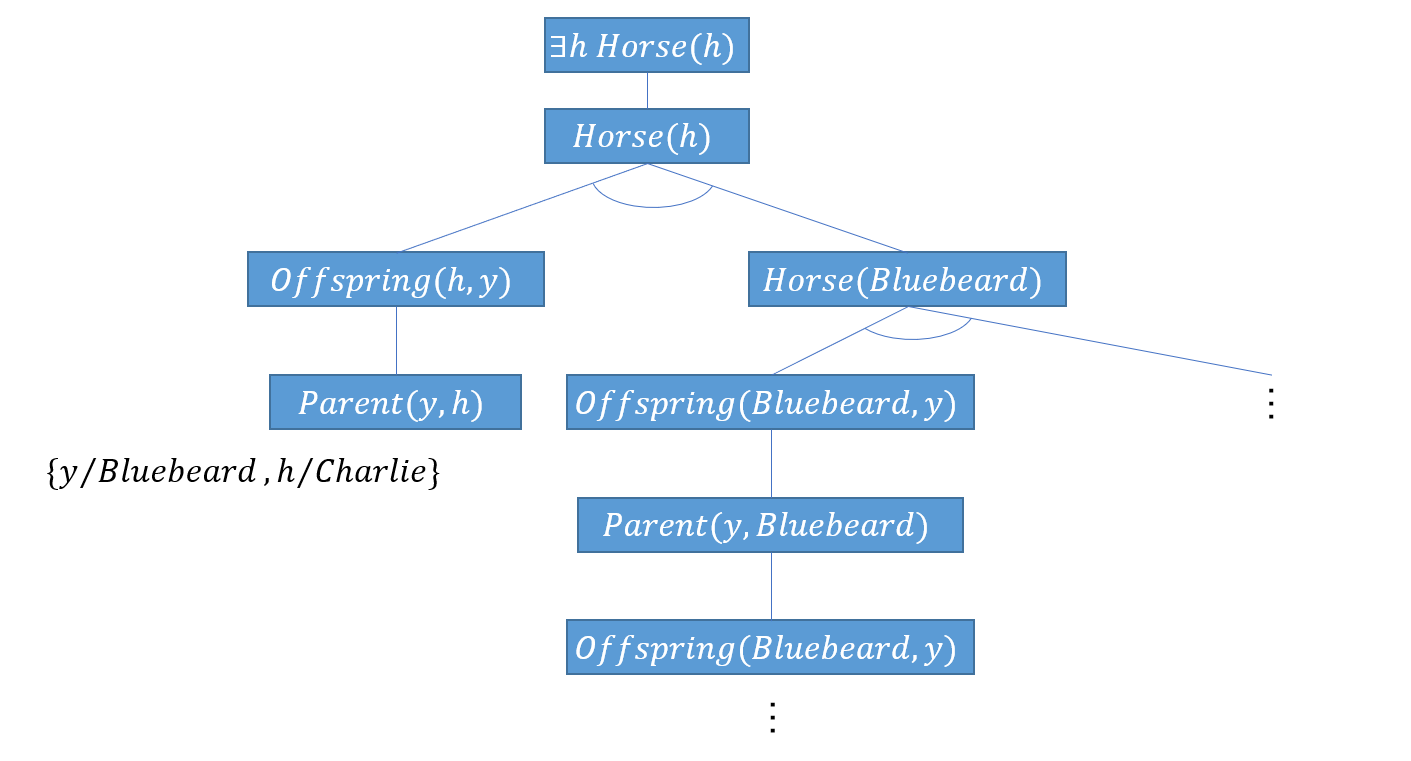
\includegraphics[width=\linewidth]{image/9.13.a.png}
	\caption{9.13.a}
\end{figure}\par

\subsection*{b.}
\noindent \textbf{What do you notice about this domain?}\\\jumpLine\noindent
如前所述, 右子树中, 由于会先用 $Offspring(x,y)\land Horse(y)\Rightarrow Horse(x)$, 因此会出现无尽的递归.
\subsection*{c.}
\noindent \textbf{How many solutions for $h$ actually follow from your sentences? }\\\jumpLine\noindent
应是 $Charlie$ 和 $Bluebeard$ 均可以为 $h$.


\end{document}




